\documentclass[10pt]{letter}
\usepackage{amsmath}
\usepackage{amsthm}
\usepackage{amssymb}
\usepackage{fullpage}
\usepackage{algorithmic}
%\usepackage{enumerate}
\usepackage{graphicx}
\usepackage{mathtools}
\DeclarePairedDelimiter{\ceil}{\lceil}{\rceil}
\DeclarePairedDelimiter{\floor}{\lfloor}{\rfloor}
%\usepackage{hyperref}
%\usepackage[]{algorithm2e}
\newcommand\tab[1][1cm]{\hspace*{#1}}
\newenvironment{solution}{\textbf{Solution:}}{\hfill$\square$}
\usepackage{amsmath,amssymb}
\makeatletter
\newsavebox\myboxA
\newsavebox\myboxB
\newlength\mylenA
\graphicspath{ {.} }
\newcommand*\xoverline[2][0.75]{%
    \sbox{\myboxA}{$\m@th#2$}%
    \setbox\myboxB\null% Phantom box
    \ht\myboxB=\ht\myboxA%
    \dp\myboxB=\dp\myboxA%
    \wd\myboxB=#1\wd\myboxA% Scale phantom
    \sbox\myboxB{$\m@th\overline{\copy\myboxB}$}%  Overlined phantom
    \setlength\mylenA{\the\wd\myboxA}%   calc width diff
    \addtolength\mylenA{-\the\wd\myboxB}%
    \ifdim\wd\myboxB<\wd\myboxA%
       \rlap{\hskip 0.5\mylenA\usebox\myboxB}{\usebox\myboxA}%
    \else
        \hskip -0.5\mylenA\rlap{\usebox\myboxA}{\hskip 0.5\mylenA\usebox\myboxB}%
    \fi}
\makeatother
\usepackage{listings}
\usepackage{color}

\definecolor{dkgreen}{rgb}{0,0.6,0}
\definecolor{gray}{rgb}{0.5,0.5,0.5}
\definecolor{mauve}{rgb}{0.58,0,0.82}

\lstset{frame=tb,
  language=Java,
  aboveskip=3mm,
  belowskip=3mm,
  showstringspaces=false,
  columns=flexible,
  basicstyle={\small\ttfamily},
  numbers=none,
  numberstyle=\tiny\color{gray},
  keywordstyle=\color{blue},
  commentstyle=\color{dkgreen},
  stringstyle=\color{mauve},
  breaklines=true,
  breakatwhitespace=true,
  tabsize=3
}
\begin{document}

\begin{center}
Assignment 2: CS 335
\end{center}

I pledge on my honor that I have not given or received any unauthorized assistance.

Name: Snehal Raj   ~~~~~~~~~~~~~~~~~~~~~~~~~~~~~~~~~~~~~~~~~~~~~~~~~~~~~~~~~~~~~~~   Roll No.:  170705     \\



\begin{enumerate}
\item 
As we see that the grammar contains left recursion, we create an equivalent grammar to avoid the same. To start, we introduce a new non-terminal namely $L'$ and then create the following grammar\\
\\
$S \rightarrow (L)|a$\\
$L \rightarrow bL'$\\
$L' \rightarrow ,SL'|SL'|\epsilon$\\

We can see that the above grammar is free from left recursion so we proceed to create the parse table. \\

To begin, we create the Fist and Follow sets of all three non-terminals which are listed below,\\
\\
$First(S) = \{c,a\}$\\
$First(L) = \{b\}$\\
$First(L') = \{ \, ,c,a,\epsilon\}$\\
\\
\\
$Follow(S) = \{\$\}$\\
$Follow(L) = \{)\}$\\
$Follow(L') = \{)\}$\\

So, having constructed the First and the Follow sets, we proceed to build the parsing table which is as shown below\\
\\
\begin{tabular}{|c|c|c|c|c|c|c|}
\hline 
• & ( & ) & a & b & \, & \$ \\ 
\hline 
S & $S\rightarrow (L)$ & • & $S\rightarrow a$ & • & • & • \\ 
\hline 
L & • & • & • & $L\rightarrow b$ & • & • \\ 
\hline 
L' & $L' \rightarrow SL'$ & $L \rightarrow \epsilon$ & $L' \rightarrow SL'$ & • & $L'\rightarrow ,SL'$ & • \\ 
\hline 
\end{tabular} 
\\
\item 
In addition to the rules mentioned, we add a dummy rule $S' \rightarrow S$ to augment the grammar. Now, following the procedure for constructing LR(1) parser, the state transitions are as follows,
\\
$I_{0}: (0) S' \rightarrow .S , \$ $\\
$(1) S \rightarrow .Lp , \$$\\
$(2) S \rightarrow .qLr , \$$\\
$(3) S \rightarrow .sr , \$$\\
$(4) S \rightarrow .qsp , \$$\\
$(5) S \rightarrow .s , p$\\
\\
\\
$goto(I_{0},S)=I_{1}:$\\
$S' \rightarrow S. ,\$$\\
\\
\\
$goto(I_{0},L)=I_{2}:$\\
$S \rightarrow L.p, \$$\\
\\
\\
$goto(I_{0},q)=I_{3}:$\\
$S \rightarrow q.Lr, \$$\\
$S \rightarrow q.sp, \$$\\
$L \rightarrow .s, r$\\
\\
\\
$goto(I_{0},s)=I_{4}:$\\
$S \rightarrow s.r, \$$\\
$L \rightarrow s., p$\\
\\
\\
$goto(I_{2},p)=I_{5}:$\\
$S \rightarrow Lp., \$$\\
\\
\\
$goto(I_{3},L)=I_{6}:$\\
$S \rightarrow qL.r, \$$\\
\\
\\
$goto(I_{3},s)=I_{7}:$\\
$S \rightarrow qs.p, \$$\\
$L \rightarrow s., r$\\
\\
\\
$goto(I_{4},r)=I_{8}:$\\
$S \rightarrow sr., \$$\\
\\
\\
$goto(I_{6},r)=I_{9}:$\\
$S \rightarrow qLr., \$$\\
\\
\\
$goto(I_{7},p)=I_{10}:$\\
$S \rightarrow qsp., \$$\\

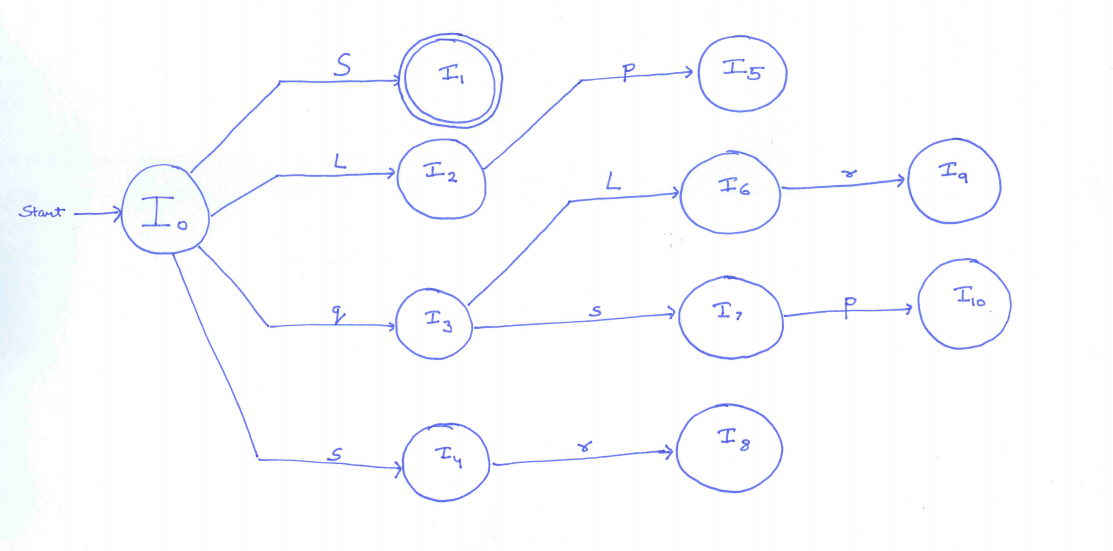
\includegraphics[scale=0.5]{dfa_2}

As, there are no conflicts and no common first components, the grammar is indeed LALR(1). The parsing table is as follows:\\
\begin{tabular}{|c|c|c|c|c|c|c|c|}
\hline 
State & Action & Action & Action & Action & Action & Action & Action \\ 
\hline 
$•$ & p & q & r & s & \$ & S & L \\ 
\hline 
0 & • & s3 & • & s4 & • & 1 & 2 \\ 
\hline 
1 & • & • & • & • & accept & • & • \\ 
\hline 
2 & s5 & • & • & • & • & • & • \\ 
\hline 
3 & • & • & • & s7 & • & • & 6 \\ 
\hline 
4 & r5 & • & s8 & • & • & • & • \\ 
\hline 
5 & • & • & • & • & r1 & • & • \\ 
\hline 
6 & • & • & s9 & • & • & • & • \\ 
\hline 
7 & s10 & • & r5 & • & • & • & • \\ 
\hline 
8 & • & • & • & • & r3 & • & • \\ 
\hline 
9 & • & • & • & • & r2 & • & • \\ 
\hline 
10 & • & • & • & • & r4 & • & • \\ 
\hline 
\end{tabular} 

Now, we follow similar procedures but do not include lookahead in items to obtain the state diagram from SLR(1) parser. The state transitions are as mentioned below\\
$I_{0}: (0) S' \rightarrow .S  $\\
$(1) S \rightarrow .Lp$\\
$(2) S \rightarrow .qLr $\\
$(3) S \rightarrow .sr $\\
$(4) S \rightarrow .qsp $\\
$(5) S \rightarrow .s$\\
\\
\\
$goto(I_{0},S)=I_{1}:$\\
$S' \rightarrow S. $\\
\\
\\
$goto(I_{0},L)=I_{2}:$\\
$S \rightarrow L.p$\\
\\
\\
$goto(I_{0},q)=I_{3}:$\\
$S \rightarrow q.Lr$\\
$S \rightarrow q.sp$\\
$L \rightarrow .s$\\
\\
\\
$goto(I_{0},s)=I_{4}:$\\
$S \rightarrow s.r$\\
$L \rightarrow s. $\\
\\
\\
$goto(I_{2},p)=I_{5}:$\\
$S \rightarrow Lp.$\\
\\
\\
$goto(I_{3},L)=I_{6}:$\\
$S \rightarrow qL.r$\\
\\
\\
$goto(I_{3},s)=I_{7}:$\\
$S \rightarrow qs.p$\\
$L \rightarrow s.$\\
\\
\\
$goto(I_{4},r)=I_{8}:$\\
$S \rightarrow sr.$\\
\\
\\
$goto(I_{6},r)=I_{9}:$\\
$S \rightarrow qLr.$\\
\\
\\
$goto(I_{7},p)=I_{10}:$\\
$S \rightarrow qsp.$\\

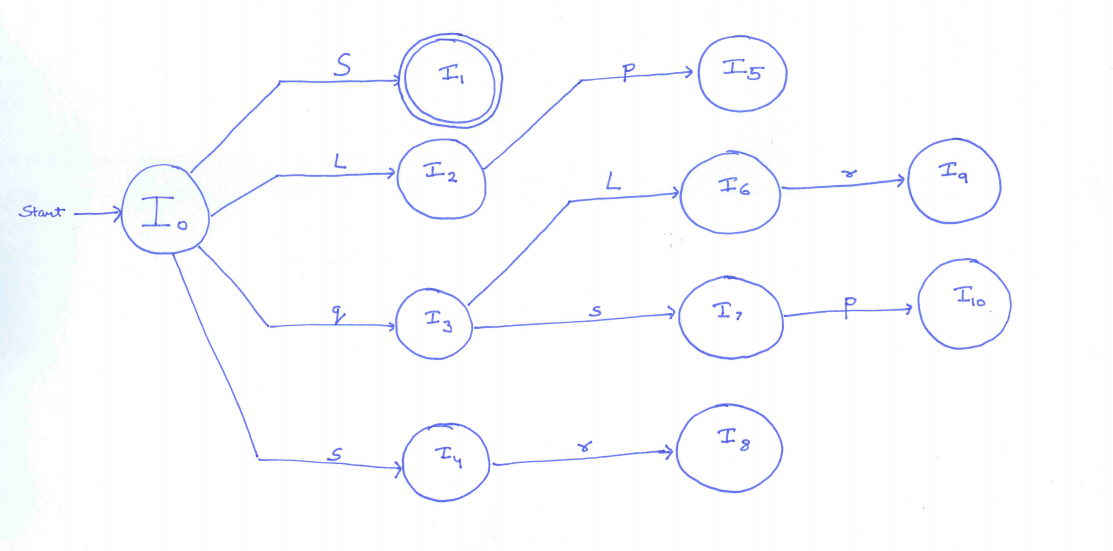
\includegraphics[scale=0.5]{dfa_2}\\
Now for this to be a SLR(1) grammar, there musn't be any conflicts while generating the parsing table. However, as we know that Follow(A)=\{a,c\}, wee that in states $I_{4}$ and $I_{7}$, there exist shift-reduce conflicts. Hence, the given grammar is not in SLR(1).

\item 
In addition to the rules mentioned, we add a dummy rule $R' \rightarrow R$ to augment the grammar. Now, following the state transition rules for the parser, the state transitions are as follows,
\\

$I_{0}: (0) R' \rightarrow .R$\\
$(1) R\rightarrow .R|R$\\
$(2) R \rightarrow .RR$\\
$(3) R \rightarrow .R*$\\
$(4) R \rightarrow .(R)$\\
$(5) R \rightarrow .a$\\
$(6) R \rightarrow .b$\\
\\
\\
$goto(I_{0},R)=I_{1}:$\\
$R \rightarrow R.$\\
$R \rightarrow R.|R$\\
$R \rightarrow R.R$\\
$R \rightarrow R.*$\\
$R \rightarrow .R|R$\\
$R \rightarrow .RR$\\
$R \rightarrow .R*$\\
$R \rightarrow .(R)$\\
$R \rightarrow .a$\\
$R \rightarrow .b$\\
\\
\\
$goto(I_{0},()=I_{2}:$\\
$R \rightarrow (.R)$\\
$R \rightarrow .R|R$\\
$R \rightarrow .RR$\\
$R \rightarrow .R*$\\
$R \rightarrow .(R)$\\
$R \rightarrow .a$\\
$R \rightarrow .b$\\
\\
\\
$goto(I_{0},a)=I_{3}:$\\
$R \rightarrow a.$\\
\\
\\
$goto(I_{0},b)=I_{4}:$\\
$R \rightarrow b.$\\
\\
\\
$goto(I_{1},|)=I_{5}:$\\
$R \rightarrow R|.R$ \\
$R \rightarrow .R|R$\\
$R \rightarrow .RR$\\
$R \rightarrow .R*$\\
$R \rightarrow .(R)$\\
$R \rightarrow .a$\\
$R \rightarrow .b$\\
\\
\\
$goto(I_{1},R)=I_{6}:$\\
$R \rightarrow RR.$\\
$R \rightarrow R.|R$\\
$R \rightarrow R.R$\\
$R \rightarrow R.*$\\
$R \rightarrow .R|R$\\
$R \rightarrow .RR$\\
$R \rightarrow .R*$\\
$R \rightarrow .(R)$\\
$R \rightarrow .a$\\
$R \rightarrow .b$\\
$R \rightarrow R*.$\\
\\
\\
$goto(I_{1},*)=I_{7}:$\\
$R \rightarrow R*.$\\
\\
\\
$goto(I_{1},()=I_{2}$\\
$goto(I_{1},a)=I_{3}$\\
$goto(I_{1},b)=I_{4}$\\
\\
\\
$goto(I_{2},R)=I_{8}:$\\
$R \rightarrow (R.)$\\
$R \rightarrow R.|R$\\
$R \rightarrow R.R$\\
$R \rightarrow R.*$\\
$R \rightarrow .R|R$\\
$R \rightarrow .RR$\\
$R \rightarrow .R*$\\
$R \rightarrow .(R)$\\
$R \rightarrow .a$\\
$R \rightarrow .b$\\
\\
\\
$goto(I_{2},()=I_{2}$\\
$goto(I_{2},a)=I_{3}$\\
$goto(I_{2},b)=I_{4}$\\
\\
\\
$goto(I_{5},R)=I_{9}$\\
$R \rightarrow R|R.$\\
$R \rightarrow R.R$\\
$R \rightarrow R.R$\\
$R \rightarrow R.*$\\
$R \rightarrow .R|R$\\
$R \rightarrow .RR$\\
$R \rightarrow .R*$\\
$R \rightarrow .(R)$\\
$R \rightarrow .a$\\
$R \rightarrow .b$\\
\\
\\
$goto(I_{5},()=I_{2}$\\
$goto(I_{5},a)=I_{3}$\\
$goto(I_{5},b)=I_{4}$\\
\\
\\
$goto(I_{6},|)=I_{5}$\\
$goto(I_{6},R)=I_{6}$\\
$goto(I_{6},*)=I_{7}$\\
$goto(I_{6},()=I_{2}$\\
$goto(I_{6},a)=I_{3}$\\
$goto(I_{6},b)=I_{4}$\\
\\
\\

$goto(I_{8},))=I_{10}$\\
$R \rightarrow (R).$\\
$goto(I_{8},|)=I_{5}$\\
$goto(I_{8},R)=I_{6}$\\
$goto(I_{8},*)=I_{7}$\\
$goto(I_{8},()=I_{2}$\\
$goto(I_{8},a)=I_{3}$\\
$goto(I_{8},b)=I_{4}$\\
\\
\\
$goto(I_{9},|)=I_{5}$\\
$goto(I_{9},R)=I_{6}$\\
$goto(I_{9},*)=I_{7}$\\
$goto(I_{9},()=I_{2}$\\
$goto(I_{9},a)=I_{3}$\\
$goto(I_{9},b)=I_{4}$\\
\\
\\
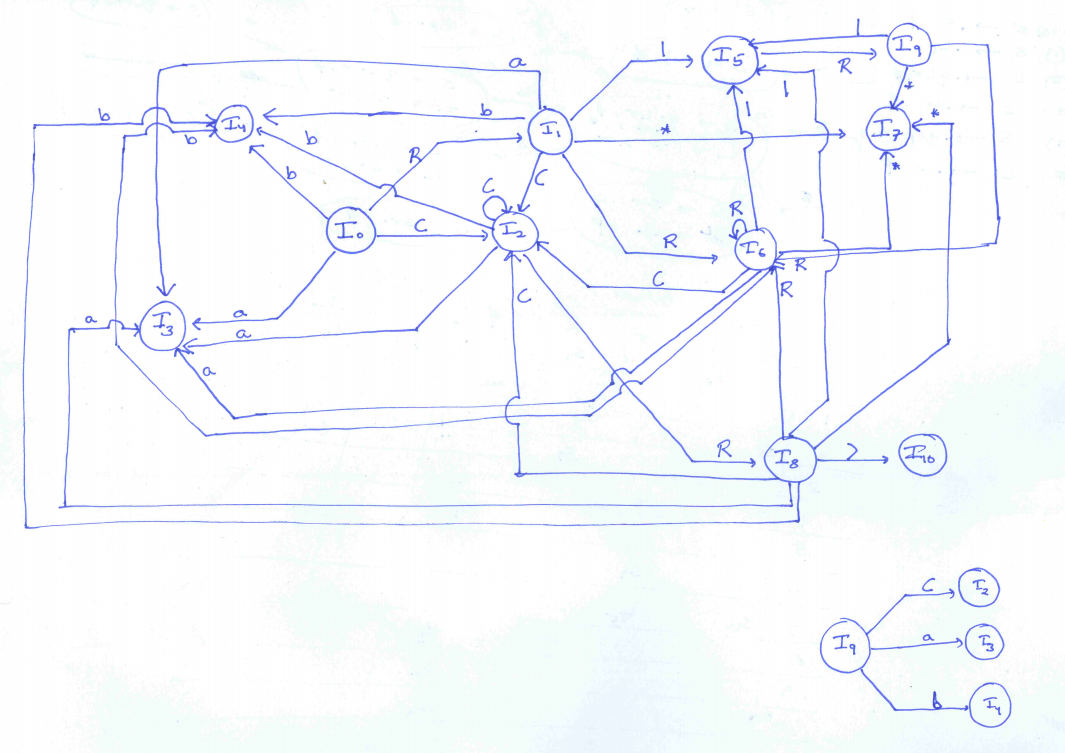
\includegraphics[scale=0.5]{dfa_3}\\
Now, we proceed to check whether there are any conflicts in the grammar. To do so, we construct the Follow set of R.\\
\\
$Follow(R) = \{|,*,(,),a,b,\$\}$\\

We see that for some states like $I_{6}$ and $I_{9}$, there are shift-reduce conflicts. So, to remove such ambiguities, we use operator precedence and associativity. The operator precedence to eliminate conflicts are as mentioned below: \\
() has higher precedence than * which has higher precedence than concatenation of RR which has higher precedence than $|$, i.e.  \\
() $>$ * $>$ concatenation $>$ $|$ \\
\\
So, using these rules we construct the parsing table as follows, \\
\\
\begin{tabular}{|c|c|c|c|c|c|c|c|c|}
\hline 
State & Action & Action & Action & Action & Action & Action & Action & Goto \\ 
\hline 
$•$ & $|$ & $*$ & $($ & $)$ & a & b & \$ & R \\ 
\hline 
0 & • & • & s2 & • & s3 & s4 & • & 1 \\ 
\hline 
1 & s5 & s7 & s2 & • & s3 & s4 & accept & 6 \\ 
\hline 
2 & • & • & s2 & • & s3 & s4 & • & 8 \\ 
\hline 
3 & r5 & r5 & r5 & r5 & r5 & r5 & r5 & • \\ 
\hline 
4 & r6 & r6 & r6 & r6 & r6 & r6 & r6 & • \\ 
\hline 
5 & • & • & s2 & • & s3 & s4 & • & 9 \\ 
\hline 
6 & r2 & s7 & r2 & r2 & r2 & r2 & r2 & 6 \\ 
\hline 
7 & r3 & r3 & r3 & r3 & r3 & r3 & r3 & • \\ 
\hline 
8 & s5 & s7 & s2 & s10 & s3 & s4 & • & 6 \\ 
\hline 
9 & r1 & s7 & s2 & r1 & s3 & s4 & r1 & 6 \\ 
\hline 
10 & r4 & r4 & r4 & r4 & r4 & r4 & r4 & • \\ 
\hline 
\end{tabular}
\item 

For generating the file lex.yy.c I have used Lex and the code snippets within Lex are written in C++
. Similarly, for the parser which is in test.y, I have written the snippets in C++.
 
I have included a script run.sh which 
\begin{itemize}
    \item Takes an input file
    \item Compiles the lex code in words.l into the c file lex.yy.c
    \item Compiles the parser in test.y 
    \item Executes the executable a.out using the grammar and lexer on the input file provided
\end{itemize}

To generate the required output file, simply run the command below  
\begin{lstlisting}
// The ouput is printed on the standard output
$ ./run.sh <INPUT-FILE>
\end{lstlisting} 
\end{enumerate}

\end{document}


